% MASTER'S LEVEL AI PRESENTATION - WEEK 1
% Course: AI for Year One Business Administration
% Lecturer: Awara Bakhtiyar Rasool
% University: Salahaddin University-Erbil
% ============================================================================

\documentclass[aspectratio=169,10pt]{beamer}

% THEME & PACKAGES
\usetheme{metropolis}
\usepackage{graphicx}
\usepackage{tikz}
\usetikzlibrary{positioning,shapes,arrows,calc,backgrounds,fit,decorations.pathreplacing,mindmap,trees,shadows}
\usepackage{amsmath,amsfonts,amssymb}
\usepackage{hyperref}
\usepackage{booktabs}
\usepackage{bm}
\usepackage{colortbl}
\usepackage{xcolor}
\usepackage{tcolorbox}
\usepackage{qrcode}

% PATHS
\graphicspath{{images/}}

% COLORS (Salahaddin University Style + Modern UI)
\definecolor{salahaddinred}{RGB}{145, 25, 25} % Approx red from logo
\definecolor{salahaddingold}{RGB}{255, 215, 0} % Approx gold from logo
\definecolor{ukhblue}{RGB}{0,51,102}
\definecolor{ukhlight}{RGB}{0,110,180}
\definecolor{forestgreen}{RGB}{34,139,34}
\definecolor{alertred}{RGB}{204,0,0}

% BEAMER COLOR CUSTOMIZATION
\setbeamercolor{title}{fg=salahaddinred}
\setbeamercolor{frametitle}{bg=salahaddinred, fg=white}
\setbeamercolor{progress bar}{fg=salahaddingold,bg=gray!20}
\setbeamercolor{palette primary}{bg=salahaddinred, fg=white}
\setbeamercolor{structure}{fg=salahaddinred}
\setbeamercolor{block title}{bg=salahaddinred,fg=white}

% CUSTOM BOXES (To make slides self-explanatory)
\newtcolorbox{info_box}[1]{colback=blue!5,colframe=ukhblue,title=#1,fonttitle=\bfseries}
\newtcolorbox{concept_box}[1]{colback=green!5,colframe=forestgreen,title=#1,fonttitle=\bfseries}
\newtcolorbox{example_box}[1]{colback=orange!5,colframe=orange!80!black,title=#1,fonttitle=\bfseries}
\newtcolorbox{quote_box}{colback=gray!5,colframe=gray!50,fonttitle=\bfseries, title=Reflection}

% FOOTER
\setbeamertemplate{footline}{
  \leavevmode%
  \hbox{%
  \begin{beamercolorbox}[wd=.4\paperwidth,ht=2.5ex,dp=1ex,left]{author in head/foot}%
    \hspace*{1em}\insertshortauthor\ |\ Salahaddin University-Erbil
  \end{beamercolorbox}%
  \begin{beamercolorbox}[wd=.6\paperwidth,ht=2.5ex,dp=1ex,right]{date in head/foot}%
    Year 1 Business Administration\hspace*{1em}\insertframenumber{} / \inserttotalframenumber\hspace*{1em}
  \end{beamercolorbox}}%
  \vskip0pt%
}
\setbeamertemplate{navigation symbols}{}

% TITLE INFORMATION
\title{Introduction to Artificial Intelligence}
\subtitle{Week 1: What, Why, and Where?}
\author{Lecturer: Awara Bakhtiyar Rasool}
\institute{
    College of Economics and Management\\
    Department of Business Administration\\
    Salahaddin University-Erbil
}
\titlegraphic{\hfill\includegraphics[height=2.5cm]{logo.png}} % Assumes logo.png is in images/
\date{\today}

\begin{document}

% ============================================================================
% TITLE & OPENING
% ============================================================================

\begin{frame}
  \titlepage
\end{frame}

\begin{frame}{Welcome to the Future}
    \begin{quote_box}
    \centering
    \textit{"Artificial Intelligence will change the world more than anything in the history of mankind. More than electricity."}\\
    \vspace{0.5em}
    \hfill — AI Expert, Dr. Kai-Fu Lee
    \end{quote_box}
    
    \begin{center}
    \textbf{Welcome to Week 1}
    \end{center}
\end{frame}

\begin{frame}{Why are we here today?}
    \textbf{Course Objectives:}
    \begin{itemize}
        \item To demystify the term "AI"
        \item To understand where it came from (History)
        \item To see how it shapes Business, Engineering, and Daily Life
    \end{itemize}
\end{frame}

% ============================================================================
% SECTION 1: WHAT IS AI?
% ============================================================================

\section{What is Artificial Intelligence?}

\begin{frame}{Defining AI}
    \begin{info_box}{Definition}
        \textbf{Artificial Intelligence (AI)} is the creation of machines that can \textbf{think}, \textbf{learn}, and \textbf{make decisions} like humans. 
    \end{info_box}
    
    \vspace{1em}
    
    It enables computers to perform tasks that typically require human intelligence, such as:
    \begin{itemize}
        \item \textbf{Visual Perception} (Seeing like a human)
        \item \textbf{Speech Recognition} (Hearing like a human)
        \item \textbf{Decision-making} (Thinking like a human)
        \item \textbf{Translation} (Communicating like a human)
    \end{itemize}
\end{frame}

\begin{frame}{The Foundations of AI}
    AI doesn't exist in a vacuum. It is built upon four major pillars:
    
    \vspace{1em}
    
    \begin{columns}[t]
        \column{0.48\textwidth}
        \begin{concept_box}{1. Mathematics}
            The language of AI.
            \begin{itemize}
                \small
                \item \textbf{Statistics}: Handling uncertainty/data
                \item \textbf{Probability}: Predicting outcomes
                \item \textbf{Calculus}: Optimizing engines
                \item \textbf{Linear Algebra}: Handling data arrays
            \end{itemize}
        \end{concept_box}
        
        \column{0.48\textwidth}
        \begin{concept_box}{2. Computer Science}
            The tools to build AI.
            \begin{itemize}
                \small
                \item \textbf{Algorithms}: Step-by-step instructions
                \item \textbf{Data Structures}: Organizing info
                \item \textbf{Programming}: Writing the code
            \end{itemize}
        \end{concept_box}
    \end{columns}
\end{frame}

\begin{frame}{The Fuel of AI: Data}
    \begin{center}
    \Large \textbf{No Data = No AI}
    \end{center}
    
    \vspace{0.5em}
    
    Just as a car needs fuel, AI needs \textbf{Data Sets}.
    
    \vspace{1em}
    
    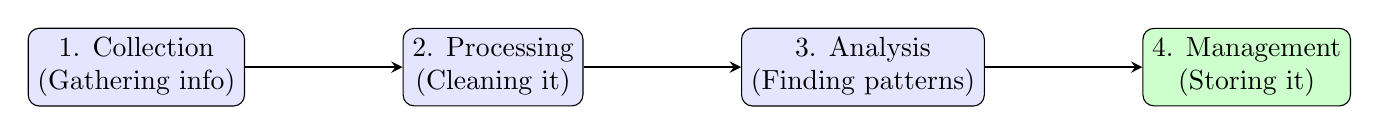
\begin{tikzpicture}[node distance=2cm, auto, >=stealth]
        % Nodes
        \node[draw, rectangle, fill=blue!10, rounded corners, align=center] (collection) {1. Collection\\(Gathering info)};
        \node[draw, rectangle, fill=blue!10, rounded corners, align=center, right=of collection] (processing) {2. Processing\\(Cleaning it)};
        \node[draw, rectangle, fill=blue!10, rounded corners, align=center, right=of processing] (analysis) {3. Analysis\\(Finding patterns)};
        \node[draw, rectangle, fill=green!20, rounded corners, align=center, right=of analysis] (mgmt) {4. Management\\(Storing it)};
        
        % Arrows
        \draw[->, thick] (collection) -- (processing);
        \draw[->, thick] (processing) -- (analysis);
        \draw[->, thick] (analysis) -- (mgmt);
    \end{tikzpicture}
    
    \vspace{1em}
    \begin{example_box}{Business Example}
    Amazon collects your purchase history (Data) $\rightarrow$ Analyzes what you like $\rightarrow$ Recommends new products (AI).
    \end{example_box}
\end{frame}

% ============================================================================
% SECTION 2: HISTORY
% ============================================================================

\section{Identify the History of AI}

\begin{frame}{Timeline of Revolution}
    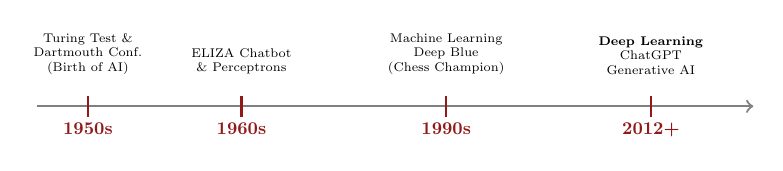
\begin{tikzpicture}[scale=0.65, transform shape]
        % Draw line
        \draw[thick, gray, ->] (0,0) -- (14,0);
        
        % 1950s
        \draw[thick, salahaddinred] (1,0.2) -- (1,-0.2) node[below] {\textbf{1950s}};
        \node[align=center, anchor=south, font=\scriptsize] at (1,0.5) {Turing Test \&\\Dartmouth Conf.\\(Birth of AI)};
        
        % 1960s
        \draw[thick, salahaddinred] (4,0.2) -- (4,-0.2) node[below] {\textbf{1960s}};
        \node[align=center, anchor=south, font=\scriptsize] at (4,0.5) {ELIZA Chatbot\\\& Perceptrons};
        
        % 1990s
        \draw[thick, salahaddinred] (8,0.2) -- (8,-0.2) node[below] {\textbf{1990s}};
        \node[align=center, anchor=south, font=\scriptsize] at (8,0.5) {Machine Learning\\Deep Blue\\(Chess Champion)};
        
        % 2010s+
        \draw[thick, salahaddinred] (12,0.2) -- (12,-0.2) node[below] {\textbf{2012+}};
        \node[align=center, anchor=south, font=\scriptsize] at (12,0.5) {\textbf{Deep Learning}\\ChatGPT\\Generative AI};
    \end{tikzpicture}
    
    \vspace{1em}
    \small
    \textbf{1950:} Alan Turing asked, "Can machines think?" (The Turing Test).\\
    \textbf{1956:} The term "Artificial Intelligence" was coined at Dartmouth Conference.\\
    \textbf{2012:} The "AlexNet" moment—Deep Learning began to dominate.
\end{frame}

\begin{frame}{Why Now? The Deep Learning Revolution}
    Why did AI suddenly boom after 2010? It wasn't magic. It was a perfect storm of three things:
    
    \vspace{1em}
    
    \begin{columns}
        \column{0.33\textwidth}
        \begin{block}{1. Big Data}
            Social media and smartphones generated massive amounts of training data.
        \end{block}
        
        \column{0.33\textwidth}
        \begin{block}{2. Better Algorithms}
            New techniques (Deep Learning, Neural Networks) mimicked the human brain better.
        \end{block}
        
        \column{0.33\textwidth}
        \begin{block}{3. GPU Power}
            Gamers' graphics cards (GPUs) turned out to be perfect for calculating AI math fast.
        \end{block}
    \end{columns}
\end{frame}

% ============================================================================
% SECTION 3: DISCIPLINES
% ============================================================================

\section{AI Disciplines \& Types}

\begin{frame}{The AI Landscape}
    AI is not one thing. It is a family of related technologies.
    \begin{center}
    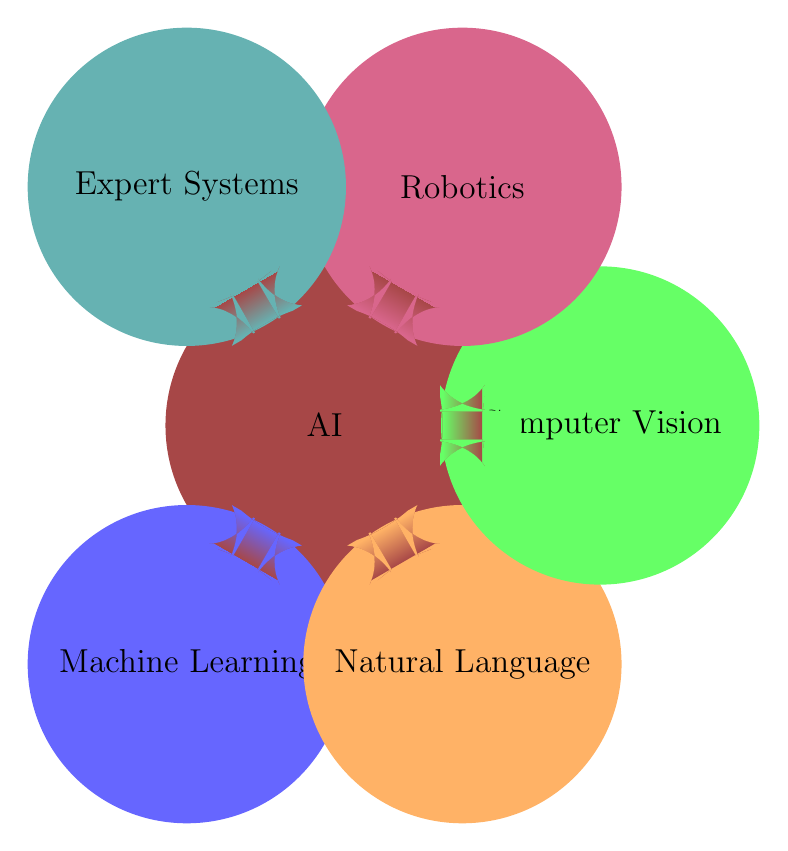
\begin{tikzpicture}[mindmap, grow cyclic, every node/.style=concept, concept color=salahaddinred!80, 
    level 1/.style={level distance=3.5cm, sibling angle=60},
    level 2/.style={level distance=2cm, sibling angle=45}]
    
    \node [root concept] {AI}
        child [concept color=blue!60] { node {Machine Learning} }
        child [concept color=orange!60] { node {Natural Language} }
        child [concept color=green!60] { node {Computer Vision} }
        child [concept color=purple!60] { node {Robotics} }
        child [concept color=teal!60] { node {Expert Systems} };
    \end{tikzpicture}
    \end{center}
\end{frame}

\begin{frame}{1. Machine Learning (ML)}
    \begin{info_box}{What is it?}
        Algorithms that allow computers to \textbf{learn from data} without being explicitly programmed for every single rule.
    \end{info_box}
    
    \textbf{Think of a child learning cats vs dogs:}
    \begin{itemize}
        \item \textbf{Old Programming:} If has\_whiskers AND says\_meow THEN cat. (Too rigid!)
        \item \textbf{Machine Learning:} Show the computer 1,000 pictures of cats and 1,000 dogs. It figures out the difference itself.
    \end{itemize}
    
    \begin{example_box}{Real World}
    Email Spam Filters: They learn what "spam" looks like from millions of emails marked by users.
    \end{example_box}
\end{frame}

\begin{frame}{2. Natural Language Processing (NLP)}
    \begin{info_box}{What is it?}
        The interaction between computers and human language. Processing, understanding, and generating text/speech.
    \end{info_box}
    
    \begin{columns}
        \column{0.6\textwidth}
        \textbf{Key Applications:}
        \begin{itemize}
            \item \textbf{Translation}: Google Translate (English $\leftrightarrow$ Kurdish)
            \item \textbf{Sentiment Analysis}: Is this customer review positive or negative?
            \item \textbf{Chatbots}: ChatGPT, Customer Service bots
        \end{itemize}
        
        \column{0.4\textwidth}
        \begin{center}
        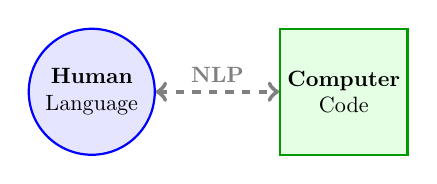
\begin{tikzpicture}[scale=0.8, every node/.style={transform shape}]
            \node[circle, fill=blue!10, draw=blue, thick, minimum size=2cm, align=center] (human) at (0,0) {\textbf{Human}\\Language};
            \node[rectangle, fill=green!10, draw=green!60!black, thick, minimum size=2cm, align=center] (computer) at (4,0) {\textbf{Computer}\\Code};
            \draw[<->, ultra thick, gray, dashed] (human) -- node[above, font=\bfseries] {NLP} (computer);
        \end{tikzpicture}
        \end{center}
    \end{columns}
\end{frame}

\begin{frame}{3. Computer Vision (CV)}
    \begin{info_box}{What is it?}
        Giving computers "eyes"—enabling them to understand digital images and videos.
    \end{info_box}
    
    \begin{example_box}{Applications}
    \begin{itemize}
        \item \textbf{FaceID}: Unlocking your iPhone with your face.
        \item \textbf{Medical}: Detecting tumors in X-rays or MRI scans.
        \item \textbf{Self-Driving Cars}: Identifying pedestrians, signs, and lanes.
    \end{itemize}
    \end{example_box}
\end{frame}

\begin{frame}{4. Robotics \& 5. Expert Systems}
    \begin{columns}
        \column{0.48\textwidth}
        \begin{concept_box}{Robotics}
            Combining AI with mechanical bodies.
            \begin{itemize}
                \item \textbf{Industrial}: Robots building cars.
                \item \textbf{Service}: Vacuum robots (Roomba).
                \item \textbf{Exploration}: Mars Rovers.
            \end{itemize}
        \end{concept_box}
        
        \column{0.48\textwidth}
        \begin{concept_box}{Expert Systems}
            AI that mimics the decision-making of a human expert.
            \begin{itemize}
                \item Used in banking for loan approval.
                \item Used in medicine for preliminary diagnosis.
                \item Follows complex "If-Then" rules derived from experts.
            \end{itemize}
        \end{concept_box}
    \end{columns}
\end{frame}

\begin{frame}{6. Neural Networks \& Deep Learning}
    \begin{info_box}{The Brain of Modern AI}
        Inspired by the biological neurons in the human brain.
    \end{info_box}
    
    \begin{itemize}
        \item \textbf{Neural Networks}: Layers of mathematical "neurons" that pass information to each other.
        \item \textbf{Deep Learning}: Neural networks with \textit{many} layers (hence "Deep").
    \end{itemize}
    
    \vspace{1em}
    \textbf{Why it matters:} This technology powers almost all the amazing AI breakthroughs we see today (GenAI, DeepFakes, AlphaGo).
\end{frame}

% ============================================================================
% SECTION 4: TYPES OF ML
% ============================================================================

\section{Types of Machine Learning}

\begin{frame}{Three Ways Machines Learn}
    \begin{columns}[t]
        \column{0.33\textwidth}
        \begin{block}{1. Supervised Learning}
            \textbf{"Learning with a Teacher"}
            \begin{itemize} \small
                \item We give the answer key.
                \item Input: Image of apple
                \item Label: "Apple"
                \item Goal: Prediction
            \end{itemize}
        \end{block}

        \column{0.33\textwidth}
        \begin{block}{2. Unsupervised Learning}
            \textbf{"Learning without a Teacher"}
            \begin{itemize} \small
                \item No labels.
                \item Goal: Find hidden patterns or groups.
                \item Ex: Customer segments.
            \end{itemize}
        \end{block}
        
        \column{0.33\textwidth}
        \begin{block}{3. Reinforcement Learning}
            \textbf{"Learning by Trial \& Error"}
            \begin{itemize} \small
                \item Training a dog (Reward/Punishment).
                \item Goal: Maximize reward.
                \item Ex: Chess, Super Mario.
            \end{itemize}
        \end{block}
    \end{columns}
\end{frame}

% ============================================================================
% SECTION 5: DETAILED ENGINEERING APPLICATIONS
% ============================================================================

\section{AI Applications in Engineering}

% MECHANICAL
\begin{frame}{1. Mechanical Engineering}
    \begin{columns}
        \column{0.6\textwidth}
        \begin{itemize}
            \item \textbf{Predictive Maintenance}: AI predicts when a machine will fail \textit{before} it happens.
            \item \textbf{Robotics}: Automating assembly lines (e.g., car manufacturing).
            \item \textbf{Simulation}: Testing designs in a virtual world to save costs.
        \end{itemize}
        \column{0.4\textwidth}
        \begin{example_box}{Project Example}
        "Optimization of rotary friction welding using finite element analysis."
        \end{example_box}
    \end{columns}
\end{frame}

% ELECTRICAL
\begin{frame}{2. Electrical Engineering}
    \begin{columns}
        \column{0.6\textwidth}
        \begin{itemize}
            \item \textbf{Smart Grids}: AI balances electricity supply and demand in real-time.
            \item \textbf{Signal Processing}: Removing noise from communication signals.
            \item \textbf{Telecommunications}: Optimizing network routing and bandwidth.
        \end{itemize}
        \column{0.4\textwidth}
        \begin{example_box}{Project Example}
        "Optimal location of STATCOM for power system voltage improvement."
        \end{example_box}
    \end{columns}
\end{frame}

% CIVIL
\begin{frame}{3. Civil Engineering}
    \begin{itemize}
        \item \textbf{Infrastructure Analysis}: Monitoring bridges and buildings for cracks using drones + AI.
        \item \textbf{Construction Mgmt}: Optimizing schedules and budgets.
        \item \textbf{Urban Planning}: Analyzing traffic flows to design better cities.
    \end{itemize}
    \begin{example_box}{Student Project}
    "Road Pothole Detection Using UAV Imagery and Deep Learning."
    \end{example_box}
\end{frame}

% ARCHITECTURE
\begin{frame}{4. Architecture \& Chemical}
    \begin{columns}[t]
        \column{0.48\textwidth}
        \textbf{Architecture:}
        \begin{itemize} \small
            \item \textbf{Generative Design}: AI explores 1000s of design options based on your constraints.
            \item \textbf{Energy Efficiency}: Designing buildings that use less power.
        \end{itemize}
        
        \column{0.48\textwidth}
        \textbf{Chemical Eng:}
        \begin{itemize} \small
            \item \textbf{Material Science}: Discovering new materials (e.g., for batteries).
            \item \textbf{Process Control}: Reducing waste in chemical plants.
        \end{itemize}
    \end{columns}
\end{frame}

% ============================================================================
% SECTION 6: OPTIMIZATION DETAILED
% ============================================================================

\section{Optimization Algorithms}

\begin{frame}{Why Optimization Matters?}
    Optimization is the "Heart" of AI training. It is used for:
    \begin{enumerate}
        \item \textbf{Model Training}: Adjusting neural network weights.
        \item \textbf{Feature Selection}: Choosing the best data inputs.
        \item \textbf{Decision Making}: Finding the best action in robotics/logistics.
        \item \textbf{Hyperparameter Tuning}: Finding the perfect settings for an algorithm.
    \end{enumerate}
\end{frame}

\begin{frame}{Famous Optimization Algorithms}
    You might hear these terms in AI research:
    
    \vspace{1em}
    
    \begin{itemize}
        \item \textbf{Gradient Descent}: The most common method. Imagine walking down a mountain blindfolded—you feel the slope and take a step down.
        \item \textbf{Genetic Algorithms (GA)}: Inspired by biological evolution (Survival of the Fittest).
        \item \textbf{Gray Wolf Optimization (GWO)}: Inspired by the hunting pack hierarchy of wolves.
        \item \textbf{Whale/Bee Optimization}: Nature-inspired algorithms for complex problems.
    \end{itemize}
\end{frame}

\begin{frame}{Real Student Projects (Previous Years)}
    \small
    \begin{itemize}
        \item \textbf{Medical}: "Falls Detection in a Wheelchair Using Wearable IMU Sensors."
        \item \textbf{Civil}: "Forecasting Failure Load of Sandstone using Gaussian Process Regression."
        \item \textbf{Electrical}: "Loss Reduction using Whale Optimization Algorithm."
    \end{itemize}
    
    \vspace{1em}
    \begin{quote_box}
    \centering \textbf{Insight:} AI is not just code. It is applied to solve REAL problems in every field.
    \end{quote_box}
\end{frame}

% ============================================================================
% CLOSING
% ============================================================================

\begin{frame}{Summary: What We Learned Today}
    \begin{enumerate}
        \item \textbf{Definition}: AI is machines mimicking human intelligence.
        \item \textbf{History}: From Turing (1950) to ChatGPT (Today). s
        \item \textbf{Types}: Machine Learning, NLP, Robotics, Vision.
        \item \textbf{Applications}: Engineering, Business, and Daily Life.
    \end{enumerate}
    
    \vspace{1em}
    \centering
    \Large \textbf{Any Questions?}
\end{frame}

\end{document}
